% !TEX TS-program = pdflatex
% !TEX encoding = UTF-8 Unicode

% This is a simple template for a LaTeX document using the "article" class.
% See "book", "report", "letter" for other types of document.

\documentclass[11pt]{article} % use larger type; default would be 10pt

\usepackage[utf8]{inputenc} % set input encoding (not needed with XeLaTeX)

%%% Examples of Article customizations
% These packages are optional, depending whether you want the features they provide.
% See the LaTeX Companion or other references for full information.

%%% PAGE DIMENSIONS
\usepackage{geometry} % to change the page dimensions
\geometry{a4paper} % or letterpaper (US) or a5paper or....
% \geometry{margin=2in} % for example, change the margins to 2 inches all round
% \geometry{landscape} % set up the page for landscape
%   read geometry.pdf for detailed page layout information

\usepackage{graphicx} % support the \includegraphics command and options
\graphicspath{{Figures/}} % Set the default folder for images

% \usepackage[parfill]{parskip} % Activate to begin paragraphs with an empty line rather than an indent

%%% PACKAGES
\usepackage{booktabs} % for much better looking tables
\usepackage{array} % for better arrays (eg matrices) in maths
\usepackage{paralist} % very flexible & customisable lists (eg. enumerate/itemize, etc.)
\usepackage{verbatim} % adds environment for commenting out blocks of text & for better verbatim
\usepackage{subfigure} % make it possible to include more than one captioned figure/table in a single float
\usepackage{cleveref}  % For referencing more than one equation at at time
\usepackage[colorlinks=true,urlcolor=blue,citecolor=blue,linkcolor=magenta]{hyperref} % for hyper referencing
\usepackage{amsmath}
% These packages are all incorporated in the memoir class to one degree or another...

%%% HEADERS & FOOTERS
\usepackage{fancyhdr} % This should be set AFTER setting up the page geometry
\pagestyle{fancy} % options: empty , plain , fancy
\renewcommand{\headrulewidth}{0pt} % customise the layout...
\lhead{}\chead{}\rhead{}
\lfoot{}\cfoot{\thepage}\rfoot{}

%%% SECTION TITLE APPEARANCE
\usepackage{sectsty}
\allsectionsfont{\sffamily\mdseries\upshape} % (See the fntguide.pdf for font help)
% (This matches ConTeXt defaults)

%%% ToC (table of contents) APPEARANCE
\usepackage[nottoc,notlof,notlot]{tocbibind} % Put the bibliography in the ToC
\usepackage[titles,subfigure]{tocloft} % Alter the style of the Table of Contents
\renewcommand{\cftsecfont}{\rmfamily\mdseries\upshape}
\renewcommand{\cftsecpagefont}{\rmfamily\mdseries\upshape} % No bold!

%%% END Article customizations

%%% The "real" document content comes below...
\title{Brownian motors thermally coupled to the environment}
\author{Jack Devine}
%\date{} % Activate to display a given date or no date (if empty),
         % otherwise the current date is printed 

\begin{document}
\maketitle

\tableofcontents

%----------------------------------------------------------------------------------------
%	ABSTRACT
%----------------------------------------------------------------------------------------
%
%\section*{Abstract} % This section will not appear in the table of contents due to the star (\section*)
%
%Brownian motors are capable of converting chemical energy directly into work and are crucial for many biological processes. The purpose of this project is to consider the motors thermal interaction with  the environment, we want to know whether these thermal interactions will change the efficiency of the Brownian motors as compared to calculations made without considering coupling to the environment.

%----------------------------------------------------------------------------------------

%\newpage % Start the article content on the second page, remove this if you have a longer abstract that goes onto the second page

%----------------------------------------------------------------------------------------
%	INTRODUCTION
%----------------------------------------------------------------------------------------

\section{Introduction}

Brownian motors are devices that can use stored energy to create directed motion on a microscopic scale, as well as being able to crank a rotor in the in the fashion of a traditional motor, they are also able to pump ions against a gradient and translocate molecules. In this project, we will model Brownian motors using concepts from statistical mechanics. In particular, a Brownian motor will be modeled by a Brownian particle diffusing over its free energy landscape \cite{Reimann2001}, which in one dimension will be denoted by $x$. In the case of Brownian motion, it is natural to think of $x$ as a spatial coordinate, however in the case of Brownian motors this is not always the case. Often we will think of $x$ as a reaction coordinate for a chemical reaction, or in the case of a rotary motor, it could be the angle of the motor. We will think of a Brownian particle moving in titled periodic potential of the form $V(x) = f x + v_0(x)$ for some external forcing $f$ and some periodic function $v_0(x)$ with period $L$. This is shown schematically in figure \ref{fig:Schematic}, in this figure we have an ensemble of  particles with a certain known density. These particles are being pushed around by thermal vibrations in a random diffusive manner, however there is also a forcing on the particles that we describe using a potential.

\begin{figure}[tb]
	\centering
	\subfigure{% 
		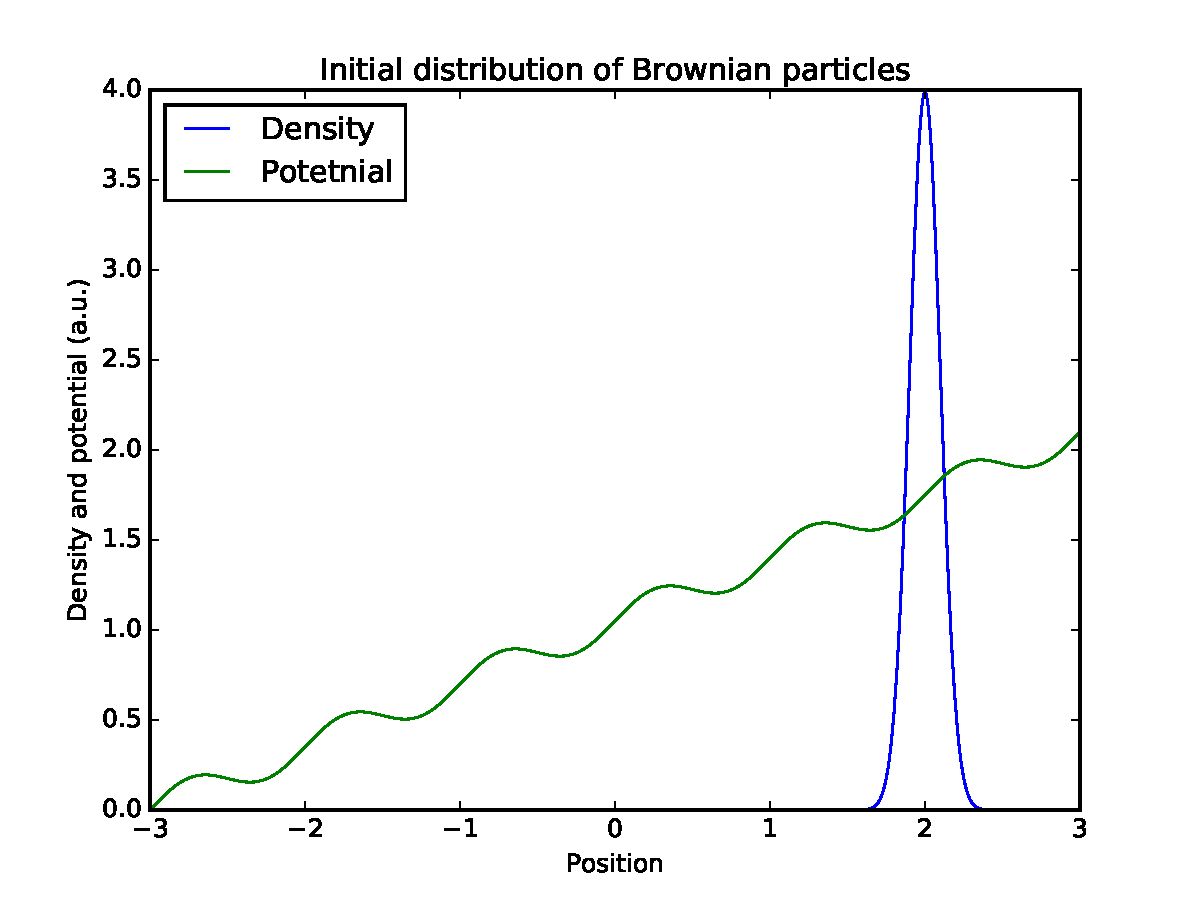
\includegraphics[width=0.45\columnwidth]{SchematicConstantTempInit}
	} 
\quad
	\subfigure{
		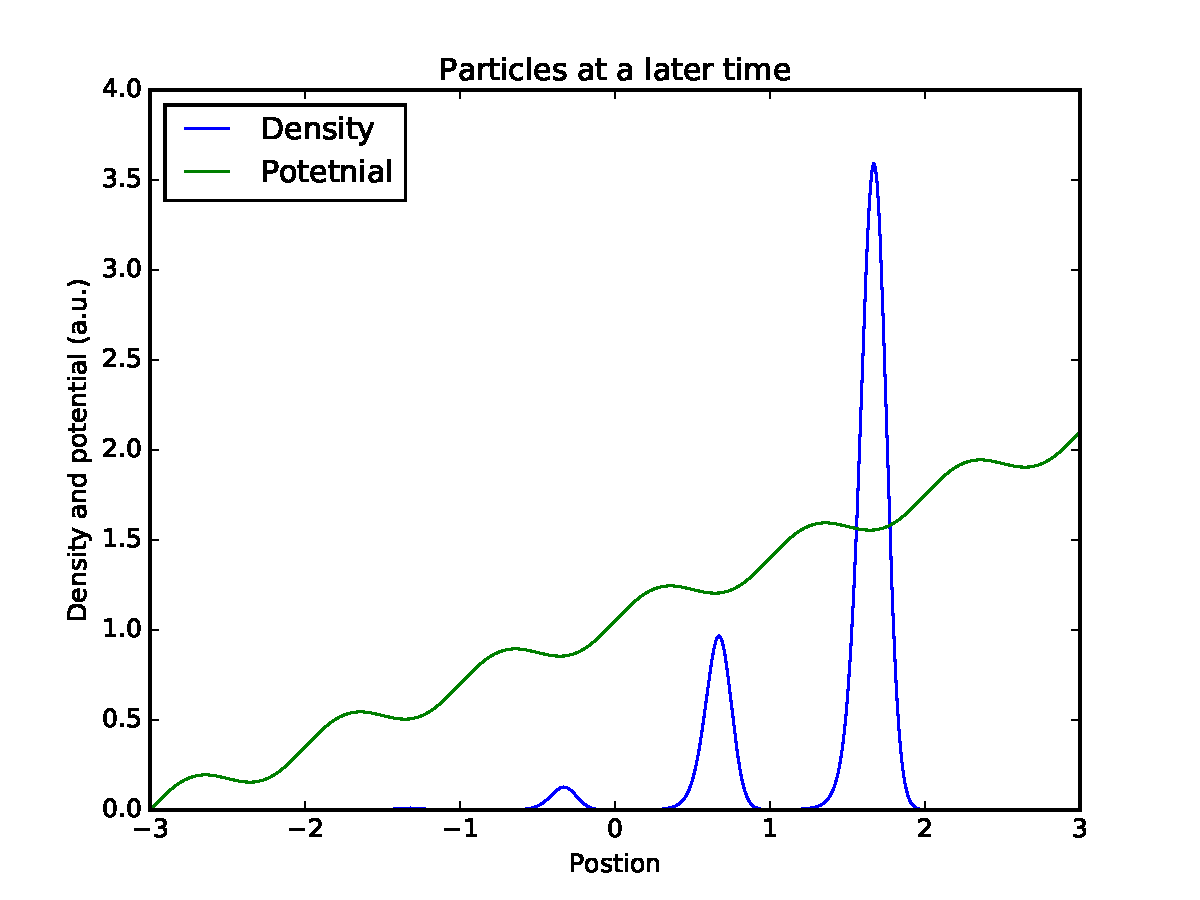
\includegraphics[width=0.45\columnwidth]{SchematicConstantTempFinal}
	}
\caption{Schematic showing particles diffusing in a one dimensional periodic potential at a fixed temperature. We see that the particles tend to drift down the potential as they diffuse, this drift will be called the current $J$ which we will quantify in section \ref{Smoluchowski}.}
\label{fig:Schematic} 
\end{figure}

As we will see, the diffusion is increased by increasing the temperature and the drift is increased by increasing $f$. In some cases such as the Landauer blowtorch, the environment has a non uniform temperature held fixed by an external heat source \cite{Landauer1988}. With this in mind, we interpret Figure \ref{fig:Schematic} as follows: Brownian particles are subject to a given potential and are agitated by thermal noise, these agitations can give the particles the energy to move over barriers as they move down the slope of the potential. As one could imagine, these thermal interactions draw energy from the environment causing the temperature of the environment to change. Normally two simplifying assumptions are made at this point \cite{Reimann2001}, (i) that the thermal fluctuations created by the motor are very small compared to the thermal energy of the surrounding environment which is assumed to be effectively infinite, (ii) that when these temperature fluctuations occur, they diffuse away so rapidly that they do not need to be accounted for. In this project, we will question the second assumption in the case of Brownian motors. It is important to note that assumption (ii) has been questioned by Streater in the context of Brownian motion \cite{Streater1997, Streater1997a}. In these articles, Streater investigates Brownian motion from a microscopic view and then comes up with a mathematical model to describe Brownian particles that are thermally coupled to the environment, he then goes on to prove that the model is thermostatistically consistent in the sense that energy is conserved and that entropy increases. We will explore a similar set of equations and we will try to determine the length scales at which the thermal coupling is important.
 
\subsection{The Smoluchowski equation coupled to the environment} \label{Smoluchowski}

The main part of this project will be trying to understand the behavior of the coupled partial differential equations given by:

\begin{eqnarray}
J(x, t) &=& \gamma^{-1} \frac{\partial}{\partial x} \left ( \frac{\partial V(x, t)}{\partial x} P(x, t) + k_B \frac{\partial}{\partial x} \left [T(x, t) P(x, t) \right] \right )  \\
\frac{\partial P(x, t)}{\partial t} &=& \frac{\partial J}{\partial x} \label{eqn:Smoluchowski} \\
\frac{\partial T(x, t)}{\partial t} &=& \frac{\partial}{\partial x} \left ( -\kappa q(x, t) + D \frac{\partial T(x, t)}{\partial x} \right ) \label{eqn:TemperatureEvolution}
\end{eqnarray} 

Where
\begin{itemize}
\item{$P(x, t)$ is the probability density as a function of time $t$  and reaction coordinate $x$}
\item{$J(x, t)$ is called the current}
\item{$\gamma$ is the friction coefficient}
\item{$V(x, t)$ is the potential for the motor}
\item{$k_B$ is the Boltzmann constant}
\item{$q(x, t) = \partial_x V(x, t) J(x, t)$ is the heat from the motor}
\item{$\kappa$ is the thermal conductivity}
\item{$D$ is the thermal diffusivity}
\end{itemize}

Equation \ref{eqn:Smoluchowski} is called the Smoluschowski equation \cite{KellerBustamante2000} and equation \ref{eqn:TemperatureEvolution} is the heat equation. These equations make our intuitive notions more precise, we see that the first term on the right hand side of the Smoluchowski equation (equation \ref{eqn:Smoluchowski}) is a drift term that is forced by our potential and that the second term contains a diffusion term that is scaled by our temperature. In fact, Figure \ref{fig:Schematic} was made by solving equation \ref{eqn:Smoluchowski} numerically. Likewise, equation \ref{eqn:TemperatureEvolution} also appeals to how our intuition of how the motor should effect its environment. The first term represents the heat flux being produced by the motor \cite{M.W.Jack2016}, while the second term represents the diffusion of temperature into the environment.

%----------------------------------------------------------------------------------------
%	PRELIMINARY RESULTS
%----------------------------------------------------------------------------------------

\section{Preliminary results}
 In order to see how these equations behave with time, we have to resort to numerical methods (see section \ref{numerics}). However we note that for a given potential there will be a stationary solution that we will refer to as the ``steady state'', given periodic boundary conditions, we will give an analytical form for this steady state. 

\subsection{Steady state solution}
In the steady state, we have: 

\begin{eqnarray}
\frac{\partial P(x, t)}{\partial t} &=&  0 \ = \ \frac{\partial J}{\partial x} \label{eqn:SmoluchowskiSteady} \\
\frac{\partial T(x, t)}{\partial t} &=& 0 \ = \ \frac{\partial}{\partial x} \left ( -\kappa q(x, t) + D \frac{\partial T(x, t)}{\partial x} \right ) \label{eqn:TemperatureSteady}
\end{eqnarray} 

Suppose that we now impose periodic boundary conditions such that $P(0, t) = P(L, t)$,  $J(0, t) = J(L, t)$ and $T(0, t) = T_0 = T(L, t)$ where $L$ is the size of one period and $T_0$ is the temperature of the bath (room temperature). Section 5.2 of \cite{Gardiner2009} gives the steady state current as:

\begin{equation}
J_s = \left [\frac{2 k_B T(L)}{\psi(L)} - \frac{2 k_B T(0)}{\psi(0)}  \right] P_s(0) \left [\int_0^L dx'/\psi(x') \right]^{-1}
\label{eqn:SteadyCurrent}
\end{equation}

with $\psi(x) \equiv \exp[-\int_0^x dx' \frac{\partial_x V(x')}{2 k_B T(x')}]$. Meanwhile, the density is:

\begin{equation}
P_s(x) = P_s(0) \left [\frac{\int_0^x \frac{dx'}{\psi(x')} \frac{T(L)}{\psi(L)} + \int_x^L \frac{dx'}{\psi(x')} \frac{T(0)}{\psi(0)} }{\frac{T(x)}{\psi(x)} \int_0^L \frac{dx'}{\psi(x')} } \right]
\label{eqn:SteadyDensity}
\end{equation}
In this case, $J_s$ is a constant and $P_s(0)$ is also a constant. Assuming that we know these constants it is now possible to find the steady state temperature. We have:

\begin{equation}
\frac{\partial T}{\partial t} = 0 =  \partial_x S_s = \kappa \partial_x V J_s - D \frac{\partial T}{\partial x}
\end{equation}
Rearranging, we find
\begin{equation}
\frac{\partial T}{\partial x} = \frac{\kappa \partial_x V J_s - \partial_x S_s}{D}
\end{equation}
Integrating both sides:
\begin{equation}
\int_0^L \frac{\partial T}{\partial x} dx = T(L) - T(0) = 0 = \frac{\kappa J_s}{D} \int_0^L \partial_x V dx - \frac{S_s}{D}L
\end{equation}

Noticing that $V(x) = v_0(x) + f x$, where $v_0(0) = v_0(L)$, we get $\int_0^L \partial_x V dx = f L$, so 

\begin{equation}
S_s = \kappa J_s f
\end{equation}

and

\begin{equation}
T(x) = T(0) + \frac{\kappa J_s}{D} \int_0^x \partial_x V dx - \frac{S_s}{D}x = T(0) + \frac{\kappa J_s}{D} (v_0(x) - v_0(0)) \label{eqn:SteadyTemperature}
\end{equation}

It would seem that one should be able to calculate the steady state current and density directly from the equations shown above. However, we notice that the constants $J_s$ and $P_s(0)$ have to satisfy equations \ref{eqn:SteadyCurrent}, \ref{eqn:SteadyDensity} and \ref{eqn:SteadyTemperature} while also satisfying the normalization condition $\int_0^L P(x) dx = 1$. To do this we define an objective function given by

\begin{equation}
obj(J_s, P_s(0)) = \left (J_s - \left [\frac{2 k_B T(L)}{\psi(L)} - \frac{2 k_B T(0)}{\psi(0)}  \right] P_s(0) \left [\int_0^L dx'/\psi(x') \right]^{-1} \right)^2  \label{eqn:Objective}
\end{equation}

And we minimize this objective function with respect to $J_s$ and $P_s(0)$ under the constraint $\int_0^L P(x) dx = 1$. Another way to do this is to guess a steady state density and temperature and use finite differencing to simulate forward in time until the transients die out.

%----------------------------------------------------------------------------------------
%	NUMERICS
%----------------------------------------------------------------------------------------

\subsection{Numerical simulation} \label{numerics}

\subsubsection{Finite differences}
The one dimensional equation can be solved on a discrete grid by using the finite differences method, the main idea behind this strategy is to approximate derivatives with equations of the form:

\begin{equation}
\frac{d f}{d x} \approx \frac{f(x - h) - f(x + h)}{2h}
\end{equation}

for some small $h$. The first thing to notice here is that our equation is ``flux conservative'', i.e. it can be written in the form 
$$ \frac{\partial P}{\partial t} = \frac{\partial J(x)}{\partial x} $$
In our case, $J(x) = \gamma^{-1} \left ( \frac{\partial V}{\partial x} P + k_B \frac{\partial}{\partial x} [T P] \right ) $. Now we will discretize space and time, we will split time into $N$ discrete times  $T_1, T_2, ..., T_n, ..., T_N$ and space into $K$ discrete points $x_1, x_2, ..., x_k, ..., x_K$. With this, we can approximate the partial derivatives that occur in our equation, first we can approximate $\frac{\partial J}{\partial x}$ with.

\begin{equation}
\left. \frac{\partial J}{\partial x} \right|_{k, n} = \frac{J_{k+1}^n - J_{k-1}^n}{2 \Delta x} + O(\Delta x^2) 
\end{equation}

And we can approximate $\frac{\partial P}{\partial t}$ with

\begin{equation}
\left. \frac{\partial P}{\partial t} \right|_{k, n} = \frac{P_k^{n+1} - P_k^n}{\Delta t} + O(\Delta t)
\end{equation}

We would like to have the equation involving $J$ written in terms of $P$, by propagating these derivatives through the definition for $J$ we get.

\begin{equation}
P_{k}^{n+1} \approx P_{k-1}^n \left [ \frac{k_B \Delta t}{2 \Delta^2} T_{k-1} - \frac{\Delta t}{2 \Delta} \partial_x V_{k-1} \right ] +
 P_k^n \left [1 - \frac{k_B \Delta t}{\Delta^2} T_k \right] +
 P_{k+1}^n \left [ \frac{k_B \Delta t}{2 \Delta^2}T_{k+1} + \frac{\Delta t}{2 \Delta} \partial_x V_{k+1} \right]
\end{equation}

Using this equation we make a matrix that has the terms multiplying $P_{k-1}^n$ as its lower off diagonal, the terms multiplying $P_k^n$ as its main diagonal and the terms multiplying $P_{k+1}^n$ as the upper diagonal. From now on we will call this matrix $A$, in order to step the distribution $P(x, t)$ forward one step (i.e. to $P(x, t + \Delta t)$), we need to use the implicit equation 

\begin{equation}
\left (I - \frac{1}{2} A \right) P_{dis}(x, t + \Delta t) \approx \left(I + \frac{1}{2}A \right)P_{dis}(x, t)
\end{equation}

where $P_{dis}$ acknowledges that $P$ has been discretized. Likewise, equation \ref{eqn:TemperatureEvolution} can be discretized to give

\begin{multline}
T^{n+1}_j \approx T^n_{j-1} \frac{\Delta t D}{2 \Delta^2} - T^n_j \left[1 + \frac{\Delta t \kappa k_B}{4 \Delta^2}(V_{j+1} - V_{j-1})(P^n_{j+1} - P^n_{j-1}) + \frac{\Delta t D}{\Delta^2} \right] + \\
 T^n_{j+1} \left [\frac{\Delta t D}{2 \Delta^2} \right] - \Delta t \kappa \left(\frac{V_{j+1} - V_{j-1}}{2 \Delta} \right )^2 P^n_j
\end{multline}

and we can form a similar implicit equation to simulate this forward in time. If we know $P(x, t)$ and $T(x, t)$ at time $t$, then we can use these methods to simulate forward in time and obtain $T(x, t + \Delta t)$ and $P(x, t + \Delta t)$.

Fortunately the matrices that we are dealing with are very sparse, so the program used to solve this equation can save on memory by calling sparse matrix libraries.

%\subsubsection{Boundary value problem in the steady state}
%Often, we will not be interested in this transient behavior and instead we will want to obtain information about the system at the steady state. To do this, we create the same matrix $A$ described above and then solve the equation
%
%\begin{equation}
%A P_s = b 
%\end{equation}
%
%Where $b$ is a vector full of zeros, but with constant entries in its first and last elements. These constants ensure the boundary condition that $P(0) = P(L)$, a similar procedure is performed to find the temperature in the steady state.
\subsubsection{Stochastic methods}
We can simulate the path of a single particle by using stochastic methods to solve the Langevin equation. By simulating many times we should be able to recover the distributions that were found through finite differencing. When simulating the system  at the microscopic level, equation \ref{eqn:Smoluchowski} becomes \cite{Reimann2001}

\begin{equation}
\gamma \dot{x}(t) = -V'(x(t)) + \xi(t)
\end{equation}

Where $\xi(t)$ is called Gaussian white noise of zero mean and has the essential properties that: $\langle \xi(t) \rangle = 0$ and $\langle \xi(t) \xi(s) \rangle = 2 \gamma k_B T \delta(t - s) $. We can also consider the stochastic equation with time discretized, in which case we get:

\begin{equation}
x(t_{n+1}) = x(t_n) - \Delta t [V'(x(t_n)) + \xi_n]/\gamma
\end{equation}

This equation can be simulated numerically, or can be used to derive Equation \ref{eqn:Smoluchowski} by taking the limit $\Delta t \to 0$ as is done in Appendix B of \cite{Reimann2001}. In the results section, we will show some results of these numerical simulations.

%----------------------------------------------------------------------------------------
%	RESULTS
%----------------------------------------------------------------------------------------
\section{Results}
Here we will show some results of finite differencing and of the stochastic methods. Figure~\ref{fig:FiniteDifferences} shows a simulation of a particle density for a certain amount of time. In this figure we see that the density tends to accumulate into the wells and that wherever the density has a sharp peak, it will interact with the environment thermally. The strength of these thermal interactions depends on $\kappa$ and for a non vanishing $D$ they tend to diffuse away into a smoother shape.

\begin{figure}[tb]
	\centering
	\subfigure{% 
		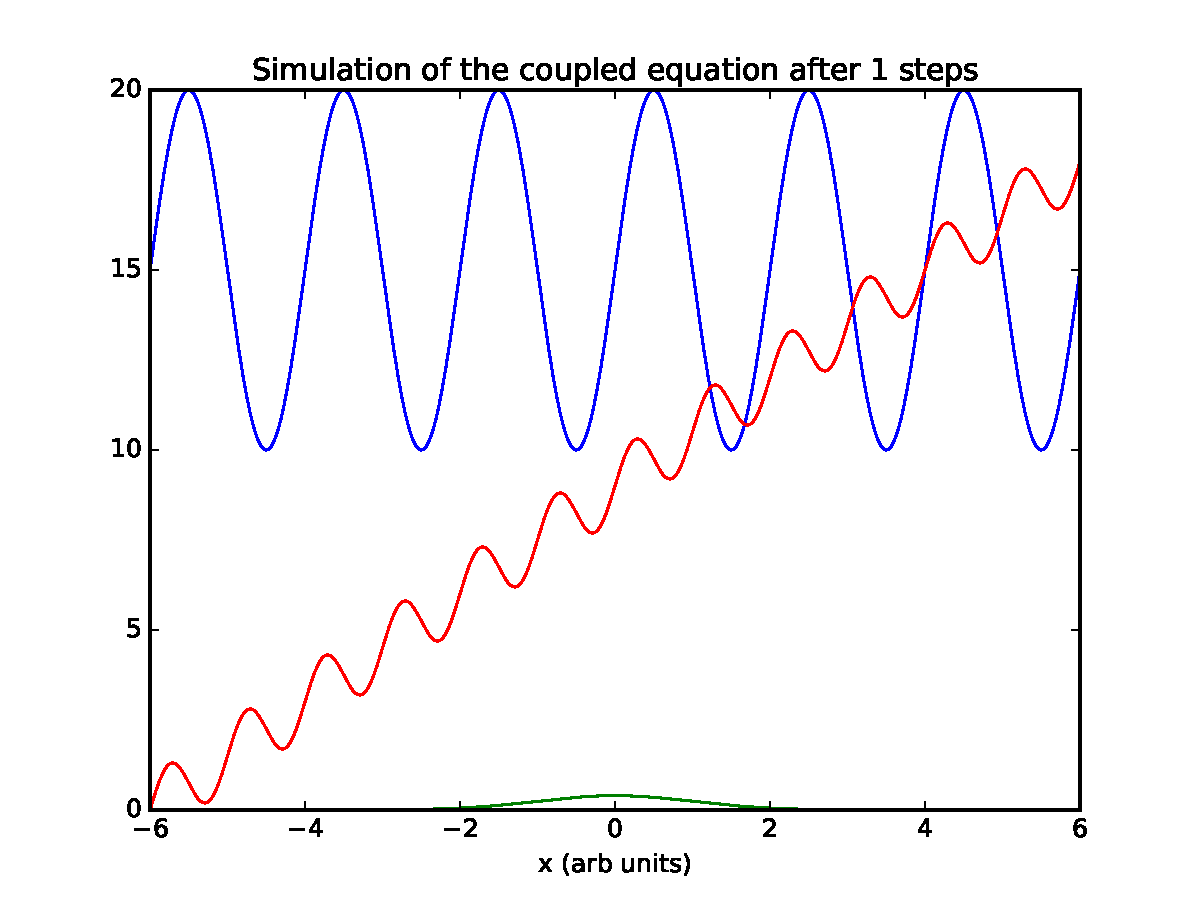
\includegraphics[width=0.45\columnwidth]{CoupledEquationFiniteDifferencesInitial}
	} 
\quad
	\subfigure{
		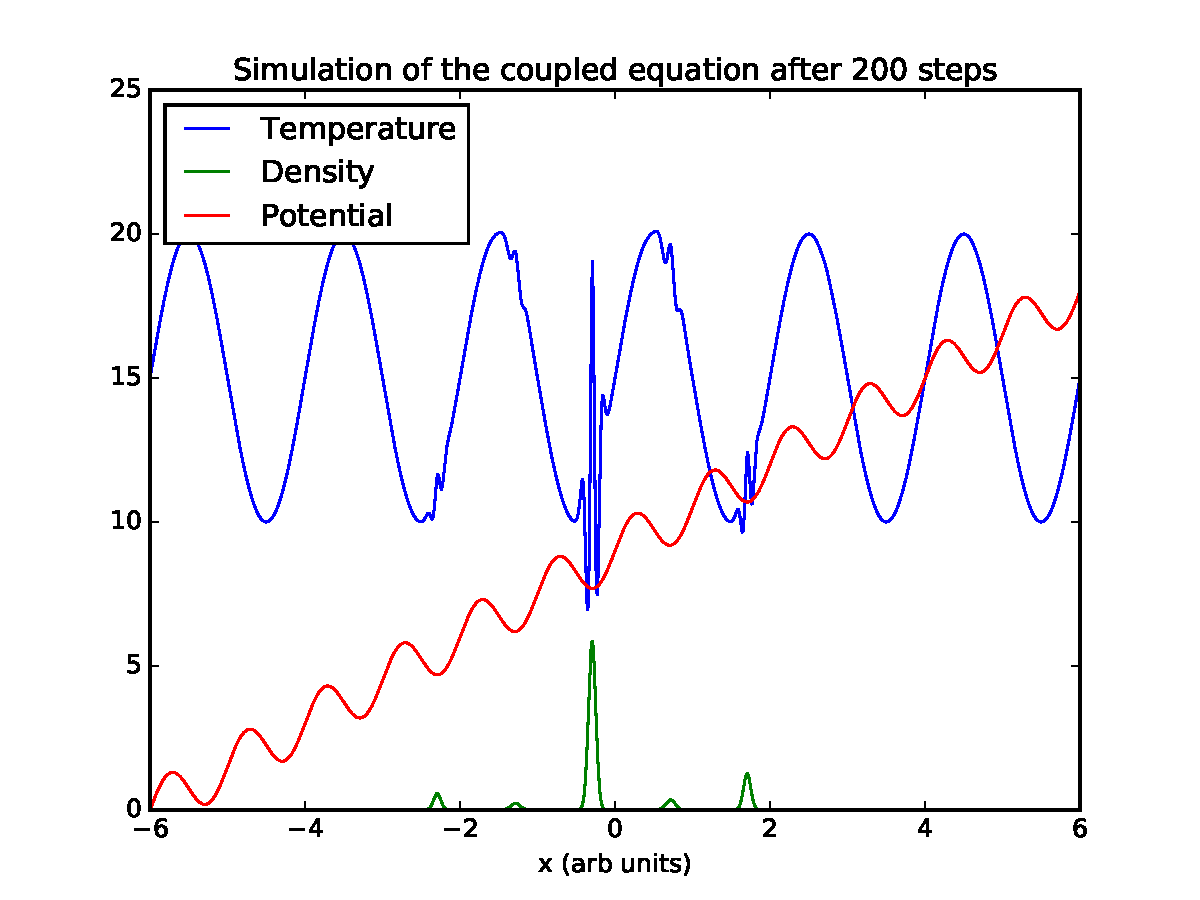
\includegraphics[width=0.45\columnwidth]{CoupledEquationFiniteDifferences}
	}
\caption{Finite differencing simulation of a distribution of particles, we see that the particles are locally interacting with the environment thermally.}
\label{fig:FiniteDifferences} 
\end{figure}

\begin{figure}[tb]
	\centering
	\subfigure{% 
		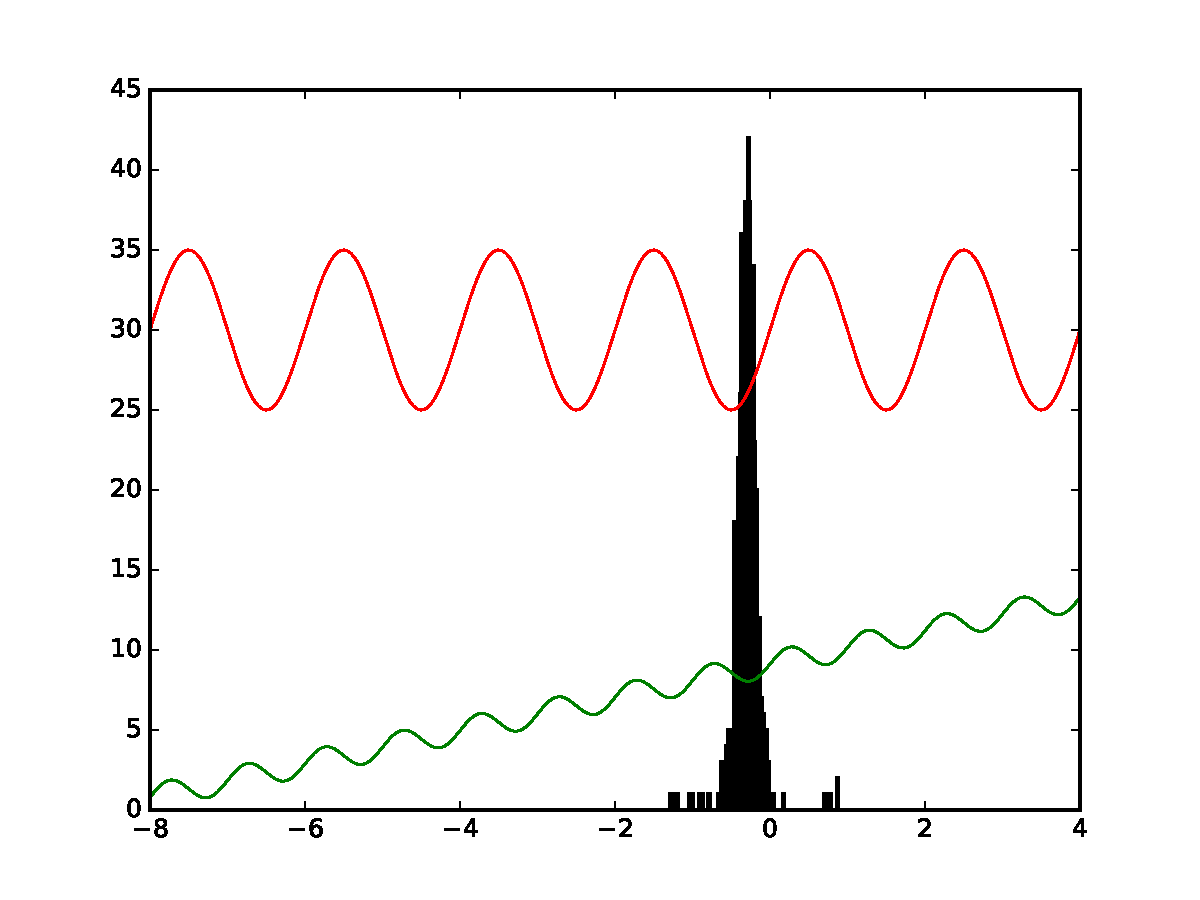
\includegraphics[width=0.45\columnwidth]{CoupledEquationStochasticInitial}
	} 
\quad
	\subfigure{
		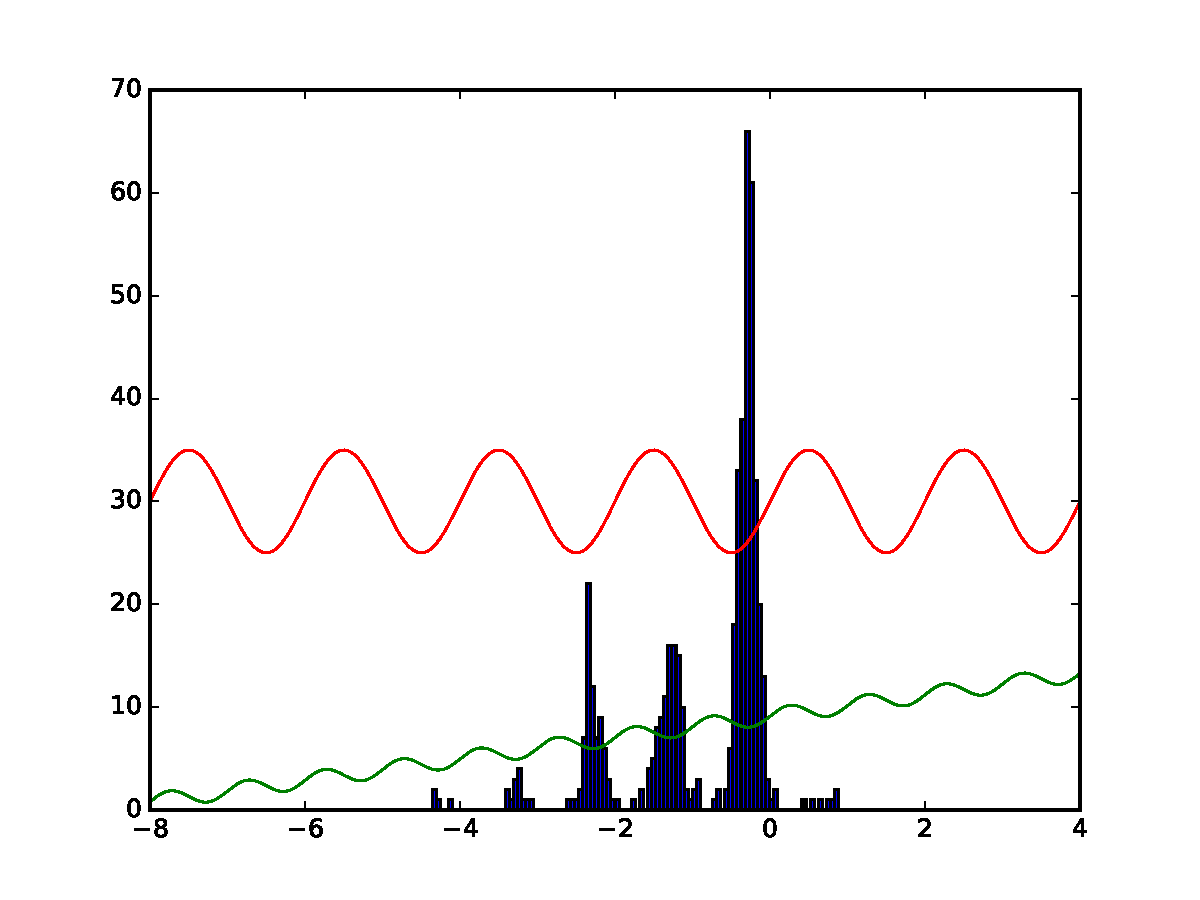
\includegraphics[width=0.45\columnwidth]{CoupledEquationStochastic}
	}
\caption{Stochastic simulation of a distribution of particles, In this simulation I have coupled the equations so that the diffusion of the particles is dependent on the temperature, however the temperature is not affected by the particles (i.e. in the case where
 $\kappa \to 0$).}
\label{fig:Stochastic} 
\end{figure}

If we allow these simulations to run for long enough, then eventually we will reach the predicted steady state.

%------------------------------------------------

%----------------------------------------------------------------------------------------
%	RESULTS AND DISCUSSION
%----------------------------------------------------------------------------------------

%------------------------------------------------

%------------------------------------------------

%----------------------------------------------------------------------------------------
%	BIBLIOGRAPHY
%----------------------------------------------------------------------------------------

%\renewcommand{\refname}{\spacedlowsmallcaps{References}} % For modifying the bibliography heading

\clearpage{}   % Make sure that the references are on a new page.
\bibliography{BibData}{} % The file containing the bibliography

\bibliographystyle{unsrt}
%----------------------------------------------------------------------------------------

\end{document}
